%\\\///\\\///\\\///\\\///\\\///\\\///\\\///\\\///\\\///\\\///\\\///\\\///\\\///\\\///\\\///\\\///\\\///\\\///\\\///
% \\//  \\//  \\//  \\//  \\//  \\//  \\//  \\//  \\//  \\//  \\//  \\//  \\//  \\//  \\//  \\//  \\//  \\//  \\//
%  \/    \/    \/    \/    \/    \/    \/    \/    \/    \/    \/    \/    \/    \/    \/    \/    \/    \/    \/
%
%       Projekt:        Bachelor Thesis
%       Autor:          Felix Dietze
%       Datum:          2011
%
%       Comment:        This is the main file
%
%  /\    /\    /\    /\    /\    /\    /\    /\    /\    /\    /\    /\    /\    /\    /\    /\    /\    /\    /\
% //\\  //\\  //\\  //\\  //\\  //\\  //\\  //\\  //\\  //\\  //\\  //\\  //\\  //\\  //\\  //\\  //\\  //\\  //\\
%///\\\///\\\///\\\///\\\///\\\///\\\///\\\///\\\///\\\///\\\///\\\///\\\///\\\///\\\///\\\///\\\///\\\///\\\///\\\

% Syntax: "\documentclass[parameter]{class}
% class: book, report, article, letter or slides
% parameter:
%       10pt | 11pt | 12pt      ~ reference value for the font size
%       oneside | twoside       ~ ..well..
%       fleqn                   ~ formulas appear left-aligned (and not centered as by default)
\documentclass[12pt,twoside,a4paper]{book}

% ========================================================================================== additional packages \/

\usepackage[utf8]{inputenc}
\usepackage{a4}         % Standard is "letter"..we want DIN A4
\usepackage{fancyhdr}   % The best package for decorating latex-documents
\usepackage{german}     % This work is in german..and everything we need for this language is in this package
\usepackage{makeidx}    % For creating the index
\usepackage{nomencl}		% Nomenclature package; formats glossary entries to show
\usepackage{color}			% Color-package
\usepackage{t1enc}			% Now we can use german letters in the "\hyphenation" - command
\usepackage{latexsym}		% Now we can use different math. symbols
\usepackage{wrapfig}		% Using for the \wrapfigure - environment to wrap text around graphics
\usepackage{amsthm}			% Now we can use \theormstyle
\usepackage{amssymb}   % AMS symbol fonts for LaTeX.

\usepackage{graphicx}
\usepackage{pslatex}
\usepackage{ifthen}

\usepackage[T1]{fontenc}
\usepackage{pslatex}

%extern packages
%\usepackage{packages/ushort}
\usepackage{psfrag}
\usepackage{subfigure}

% \usepackage{amsfonts}  % TeX fonts from the American Mathematical Society.
% \usepackage{array}     % Arrays and tables with formatted columns.
% \usepackage{enumerate} % Adds an optional argument to the enumerate-env. which det. the style of the counter.
% \usepackage{eepic}     % Extensions to epic and the LaTeX drawing tools
% \usepackage{epic}      % Apackage enhancing LaTeX's picture mode
% \usepackage{ifthen}    % Conditionals in LaTeX2e documents.
% \usepackage{longtable} % Support for tables longer than a page.
% \usepackage{theorem}   % An extension to "\newtheorem"-structure%\usepackage{packages/mm}% ???

\usepackage{listings}  % Typeset source code listings using LaTeX.
\lstloadlanguages{C++}
\lstset{language=C++}

% \usepackage[dvips]{graphicx}
% \usepackage{wrapfig}
% \usepackage{psfrag}
% \usepackage{amsthm}
% \usepackage{amssymb}
% \usepackage{url}
% \usepackage{alltt}


% ================================================================================================ preprocessing \/

% ============================================================ style definitions and declarations \/

%%%
% Footer and header
%%%
\setlength{\headheight}{14.5pt}
\addtolength{\headwidth}{0.5\marginparwidth}
\lhead[\fancyplain{}{\thepage}]{\fancyplain{}{\nouppercase{\sffamily\rightmark}}}
\rhead[\fancyplain{}{\nouppercase{\sffamily\leftmark}}]{\fancyplain{}{\thepage}}

%%%
% Hyphenation
%%%
\hyphenation{FAVOuR quader-förmige}


% ================================================================================== new commands \/

%%%
% Adding a completely blank page (no footer, no header)
%%%
\newcommand{\blankpage}
{
  \clearpage{\pagestyle{empty}\cleardoublepage}
}

%%%
% Graphicspath (not needed yet)
%%%
\graphicspath{
	{pictures/}
}

%%%
% New commands for including graphics
%%%
\setlength{\fboxsep}{0.3cm}		% Separation between the framebox and the room inside !
\newlength{\gw}					% New lentgh for the width of the graphic !

\newcommand{\graphik}[2][1]{\includegraphics[width=#1\gw]{#2}}

\newcommand{\rahmengraphik}[2][1]
{
	\setlength{\gw}{#1\textwidth}
	\addtolength{\gw}{-2\fboxsep}
	\addtolength{\gw}{-2\fboxrule}
	\centering
        \graphik{#2}
%%	\framebox[#1\textwidth]{\graphik{#2}}
}

%%%
% Listingsdefinitions
%%%

\definecolor{black_color}{rgb}{0.0,0.0,0.0}
\definecolor{listingbgr_color}{rgb}{1.0,1.0,0.9}
\lstset{basicstyle=\small}
\lstset{stringstyle=\ttfamily}
\lstset{backgroundcolor=\color{listingbgr_color}}
\lstset{framesep=0.3cm}
\lstset{frame=single}
\lstset{captionpos=b}
\lstset{tabsize=2}
\lstset{abovecaptionskip=0.5cm}
\renewcommand{\lstlistlistingname}{Listingsverzeichnis}

%%%
% We want also subsubsections to be enumerated
%%%
\setcounter{secnumdepth}{3}
\setcounter{tocdepth}{3}


%%%
% Prepare the environment for definitions
%%%
\theoremstyle{definition}
\newtheorem{definition}{Definition}[chapter]
\newtheorem{theorem}{Satz}[chapter]


\makeglossary
%\makeindex

% ==================================================================================================== main part \/
\begin{document}

% ======================================================================= FRONT PART OF THE BOOK \/
\frontmatter

% ============================================================================== titel \/
%\\\///\\\///\\\///\\\///\\\///\\\///\\\///\\\///\\\///\\\///\\\///\\\///\\\///\\\///\\\///\\\///\\\///\\\///\\\///
% \\//  \\//  \\//  \\//  \\//  \\//  \\//  \\//  \\//  \\//  \\//  \\//  \\//  \\//  \\//  \\//  \\//  \\//  \\//
%  \/    \/    \/    \/    \/    \/    \/    \/    \/    \/    \/    \/    \/    \/    \/    \/    \/    \/    \/
%
%       Projekt:        Bachelor Thesis
%       Autor:          Felix Dietze
%       Datum:          2011
%
%       Comment:        Here is the definition of the titlepage
%
%  /\    /\    /\    /\    /\    /\    /\    /\    /\    /\    /\    /\    /\    /\    /\    /\    /\    /\    /\
% //\\  //\\  //\\  //\\  //\\  //\\  //\\  //\\  //\\  //\\  //\\  //\\  //\\  //\\  //\\  //\\  //\\  //\\  //\\
%///\\\///\\\///\\\///\\\///\\\///\\\///\\\///\\\///\\\///\\\///\\\///\\\///\\\///\\\///\\\///\\\///\\\///\\\///\\\

\begin{titlepage}

\begin{center}

\parbox{8cm}{
\includegraphics[height=1.6cm]{title/logo_rwth_color}}
\hfill
\parbox{2.5cm}{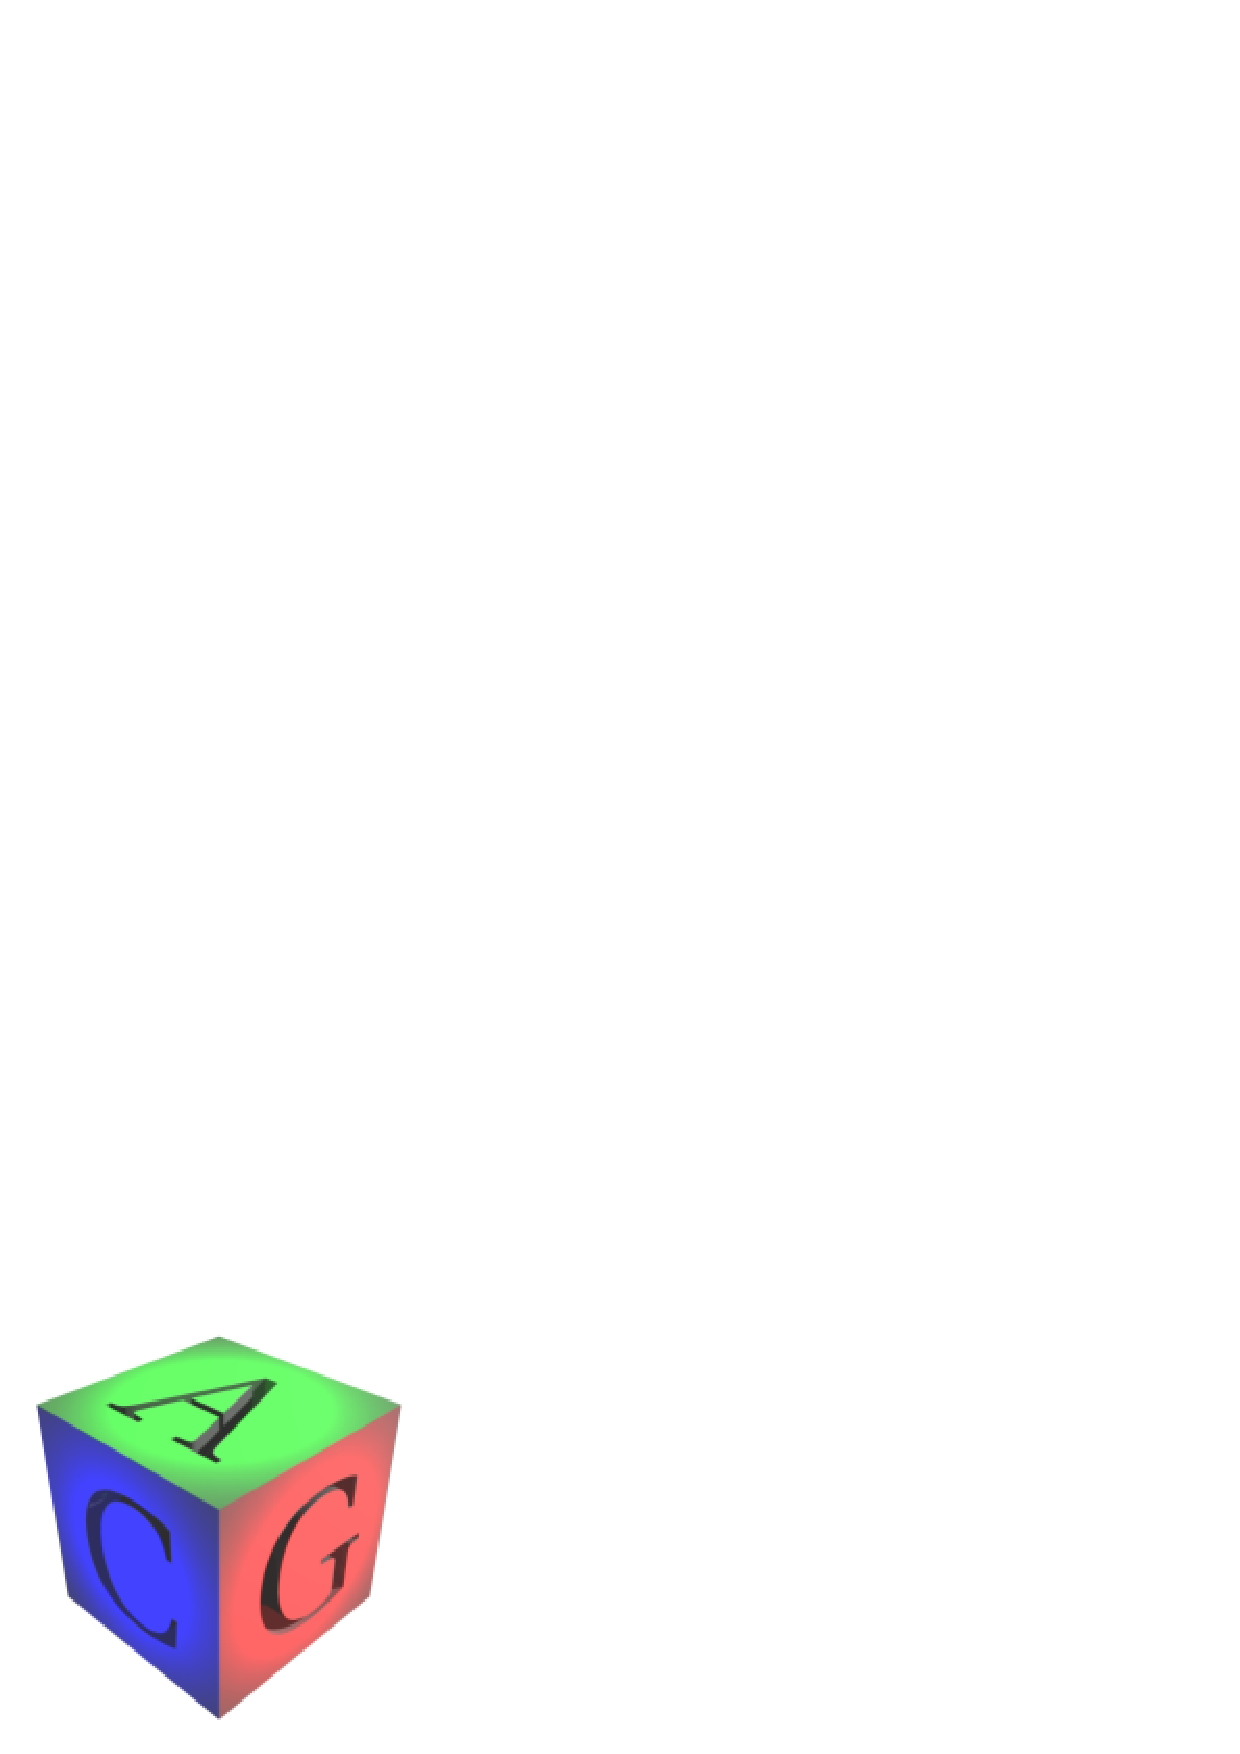
\includegraphics[width=2.3cm]{title/logo_acg_color}}

\vspace{0.5cm}

\vspace{0.75cm}

\textsf
{
Fakultät für Mathematik, Informatik und Naturwissenschaften\\
Lehrstuhl für Informatik VIII (Computergraphik und Multimedia)\\
Prof. Dr. Leif Kobbelt
}

\rule{\linewidth}{1pt}

\vspace{1.75cm}
\LARGE
\textbf{Bachelorarbeit}

\vspace{1.7cm}
\huge
Vorhersage und Interaktive Komposition von Noise-Funktionen zum Rendern Unbeschränkter Prozeduraler Welten in Echtzeit

\vspace{2.0cm}
\Large
Felix Dietze\\
\large
Matrikelnummer: 290734

\vspace{0.5cm}
August 2011

\vspace{1.05cm}
\rule{\linewidth}{1pt}

\vspace{0.5cm}
\textsf{\textbf{
\normalsize
\begin{tabular}{ll}
Erstgutachter:  & Prof. Dr. Leif Kobbelt\\
Zweitgutachter: & xxxxxxxxxxxxx\\
\end{tabular}
}}
\end{center}

\end{titlepage}


% ========================================================================= empty page \/
% \blankpage

% ==================================================================== acknowledgement \/
% \include{acknowledgement}

% ========================================================================= empty page \/
\blankpage

% ========================================================================= dedication \/
%\include{dedication}

% ========================================================== Eidesstattliche Erklärung \/
%\\\///\\\///\\\///\\\///\\\///\\\///\\\///\\\///\\\///\\\///\\\///\\\///\\\///\\\///\\\///\\\///\\\///\\\///\\\///
% \\//  \\//  \\//  \\//  \\//  \\//  \\//  \\//  \\//  \\//  \\//  \\//  \\//  \\//  \\//  \\//  \\//  \\//  \\//
%  \/    \/    \/    \/    \/    \/    \/    \/    \/    \/    \/    \/    \/    \/    \/    \/    \/    \/    \/
%
%	Projekt:	Bachelor Thesis
%	Autor:	    Felix Dietze
%	Datum:		2011
%
%	Comment:	Affirmation
%
%  /\    /\    /\    /\    /\    /\    /\    /\    /\    /\    /\    /\    /\    /\    /\    /\    /\    /\    /\
% //\\  //\\  //\\  //\\  //\\  //\\  //\\  //\\  //\\  //\\  //\\  //\\  //\\  //\\  //\\  //\\  //\\  //\\  //\\
%///\\\///\\\///\\\///\\\///\\\///\\\///\\\///\\\///\\\///\\\///\\\///\\\///\\\///\\\///\\\///\\\///\\\///\\\///\\\

\pagestyle{fancyplain}

\begin{figure}
I hereby affirm that I composed this work independently and used no other than the specified sources and tools and
that I marked all quotes as such.
\bigskip

Hiermit versichere ich, diese Arbeit selbst\"andig verfasst und keine anderen als die angegebenen Quellen und
Hilfsmittel benutzt, sowie Zitate kenntlich gemacht zu haben.
\medskip

\begin{flushright}
Aachen, den \today

\vspace{1.5cm}
\small
(Felix Dietze)
\end{flushright}
\end{figure}

%\clearpage
%\thispagestyle{empty}
%\ \\[3cm]
%\begin{center}
%\parbox{10cm}
%{ 
%Eidessstattliche Erklärung: \newline\newline
%Ich versichere, dass ich die vorliegende Arbeit selbständig verfaßt und keine anderen als die angegebenen
%Quellen und Hilfmittel benutzt habe.
%\\[8mm] 
%Aachen, den \today
%}
%\end{center}


% ========================================================================= empty page \/
\blankpage

% ========================================================================= abstract \/
\chapter{Zusammenfassung}
Beschreibung des Noise-Editors
Prediction über Intervall-Arithmetik und konvexer Hülle von Bezier-Kurven


% =========================================================================== CONTENTS \/
{ % changing "parskip" only here
% \setlength{\parskip}{0.2ex plus0.1ex minus0.1ex}

\pagestyle{fancyplain}
\tableofcontents
\newpage

% \listoffigures
% \addcontentsline{toc}{chapter}{Abbildungsverzeichnis}
% 
% \listoftables
% \addcontentsline{toc}{chapter}{Tabellenverzeichnis}
% 
% \lstlistoflistings
% \addcontentsline{toc}{chapter}{Listingsverzeichnis}
}

% ======================================================================== MAIN PART OF THE BOOK \/
\mainmatter

\chapter{Einleitung}
%%\begin{figure}[ht!]
%%\rahmengraphik[0.5]{01/bla.eps}
%%\caption{ Beispiel }
%%\label{bsp_label}
%%\end{figure}
- Perlins Original-Noise-Paper und die ersten ansätze für Noise-Funktions-Kompositionen
- Prozedurale Textur-Node-Editoren
- Intervallarithmetik im Ray-Casting

\chapter{Noise-Editor}
\section{Motivation}
Prozedurale Welten können durch Kompositionen von Dichtefunktionen beschrieben werden. Im gängigen Workflow wird eine solche Komposition in der Programmiersprache des Renderers geschrieben, kompiliert, das Programm gestartet und das Resultat betrachtet. Entspricht das Ergebnis nicht den Erwartungen wird der Code angepasst und die restlichen Schritte erneut ausgeführt. Jede dieser Iterationen nimmt viel Zeit in Anspruch und führt bei komplexeren Kompositionen erst nach sehr langer Zeit oder nicht zu sinnvollen Ergebnissen.

Um das Entwerfen von prozeduralen Welten zu beschleunigen, habe ich ein Werkzeug entwickelt, mit dem es innerhalb kürzester Zeit möglich ist, Funktionen zu komponieren, deren Parameter zu ändern und das Ergebnis in Echtzeit betrachten zu können.

\section{Anforderungen}
Dem Noise-Editor unterliegen einige Anforderungen, um den Workflow drastisch verbessern zu können:
\begin{enumerate}
	\item Es muss die Komposition beliebiger Funktionen möglich sein.
	\item Änderungen der Kompositionsschachtelung müssen in Echtzeit angezeigt werden.
	\item Änderungen der Parameter einer Funktion müssen in Echtzeit angezeigt werden.
	\item Sollte keine passende Integrierte Funktion für einen Anwendungsfall bereit stehen, muss es die Möglichkeit geben, eigenen Code eingeben zu können.
	\item Eine Prozedurale Welt besteht aus Formen (Dichte) und Materialien. Diese zwei Aspekte müssen modellierbar sein.
	\item Es muss Code in der Sprache des Renderers exportiert werden können um, nahtlos mit jedem beliebigen Renderer arbeiten zu können.
	\item Für Kompositionen im $\mathbb{R}^3$ muss in der Vorschau die Tiefe wahrnehmbar sein.
\end{enumerate}

\section{Umsetzung}
Die oben erwähnten Anforderungen lassen sich mit einem Node-Editor wie folgt modellieren:

Jeder Node entspricht einer Funktion. Daher besitzt jeder Node Eingänge für Argumente und einen Ausgang für den Funktionswert. Besteht eine Verbindung zwischen dem Ausgang eines Nodes und dem Eingang eines anderen Nodes entspricht dies einer Komposition der beiden Funktionen. Konstante Argumente entsprechen Schiebereglern auf einem Node. Es existieren weitere Nodes um die Verarbeitung der Komposition zu modellieren (Vorschau), die Weltkoordinaten in Funktionen einsetzen zu können (Quellen) und ein Node zur Eingabe von eigenem Code. Zudem enthält der Vorschau-Node zwei Eingange für Material und Dichte.

Jedem Node unterliegt Programmcode für die darstellende Funktion. Aus diesen Codeteilen kann über den Kompositionsbaum Code für den Renderer generiert werden.

Die fehlenden Punkte für Echtzeit- und Tiefen-Vorschau sind abhängig von der Implementierung des Editors und werden in Sektion \ref{architecture} behandelt.

\section{Softwarearchitektur}
\label{architecture}
\subsection{Graphische Oberfläche und Organisation der Nodes}
\subsection{Verwaltung der Verbindungen, Code-Generierung und Echtzeit-Vorschau}





%	- Architektur des Noise-Node-Editors
%		- Scala/Swing, Components
%		- Traits für Eigenschaften/Features von Swing-Componenten (Resize, Move, ScrollZoom)
%		- Event-Fluss
%		- Definition von Nodes/Kategorien
%			- Instanz eines Nodes als Swing-Komponente
%		- Verbindung von Nodes
%			- unterliegende Datenstruktur
%			- Konnektoren und Datentypen
%				- (Keine Listen, d.h. Gruppierung von Argumenten, wegen Komplexität der Codegenerierung und Performance-Problemen)
%		- Code-Generierung
%			- Module für unterschiedliche Anwendungszwecke
%			- Baum-Modell für beliebige Sprachen
%			- Beispielgenerierung: Scala-Code
%		- Echtzeit-Vorschau durch Laufzeit-Compilierung von generiertem Code
%			- Interpreter-Warteschlange
%			- Binden von Slider-Werten an compilierten Code
%			- Interpretierte Formeln für Slider
%		- Weitere Features
%			- Custom-Nodes
%			- Perspektiven
%			- Verschiedene Ansichten der Preview, u.a. Tiefen-Ansicht, Normalisierung
%			- Materialien
%			- Laden/Speichern von Kompositionen mit XML
%			- Verschiebbarkeit/Scrollbarkeit der Arbeitsfläche
%	- Interessante Kompositionen
%		- Oberfläche
%		- Gesteinsschichten
%		- Verzerrung durch Noise
%		- Technodots
%		- Schachbrett-Muster
%		- ...?
%	- Anwndungsbeispiele
%		- Game-Engine
%		- ...?

\chapter{Vorhersage von Kompositionen}
%%\begin{figure}[ht!]
%%\rahmengraphik[0.5]{01/bla.eps}
%%\caption{ Beispiel }
%%\label{bsp_label}
%%\end{figure}
	- Intervall-Vorhersage durch Intervallarithmetik
		- Intervallarithmetik auf einfachen Funktionen
		- Intervallarithmetik für Improved Perlin Noise
			- Perlin-Noise ist Polynom
			- Polynome lassen sich in Bezierkurven mit regelmäßiger Anordnung der Kontrollpunkte umrechnen
			- Bezierkurven lassen sich leicht zerschneiden
			- Bezierkurven liegen in der Konvexen hülle der Kontrollpunkte
			- Das Minimum und Maximum der Kontrollpunkte bestimmt den zu erwartenden Wertebereich.
			- Implementierung
		- Vorhersage in der GameEngine
			- Bereichsanfrage von Oktanten
			- Kontrollpunkt-cache in der Noise-Prediction
			- Vorhersage-Code-Generierung mit dem Noise-Editor

\chapter{Resultate}
%%\begin{figure}[ht!]
%%\rahmengraphik[0.5]{01/bla.eps}
%%\caption{ Beispiel }
%%\label{bsp_label}
%%\end{figure}
- Perlins Original-Noise-Paper und die ersten ansätze für Noise-Funktions-Kompositionen
- Prozedurale Textur-Node-Editoren
- Intervallarithmetik im Ray-Casting

\chapter{Zukunft}
%%\begin{figure}[ht!]
%%\rahmengraphik[0.5]{01/bla.eps}
%%\caption{ Beispiel }
%%\label{bsp_label}
%%\end{figure}
	- Affine Arithmetik für die Vorhersage
	- Ausweitung der Modulfähigkeiten im NoiseEditor

% ========================================================================= empty page \/
\blankpage

% Footer and header extra for introduction
% \lhead[\fancyplain{}{\thepage}]{\fancyplain{}{\nouppercase{\sffamily Einleitung}}}
% \rhead[\fancyplain{}{\nouppercase{\sffamily Einleitung}}]{\fancyplain{}{\thepage}}

% \addcontentsline{toc}{chapter}{Einleitung}
% \include{chapters/00_introduction}

% Footer and header back to standard
% \lhead[\fancyplain{}{\thepage}]{\fancyplain{}{\nouppercase{\sffamily\rightmark}}}
% \rhead[\fancyplain{}{\nouppercase{\sffamily\leftmark}}]{\fancyplain{}{\thepage}}

% \include{chapters/01_meshreconstruction}
% \include{chapters/02_poly}
% \include{chapters/03_volume}
% \include{chapters/04_polyagain}
% \include{chapters/05_outputoptimization}
% \include{chapters/06_conclusions}

% ======================================================================== BACK PART OF THE BOOK \/
\backmatter

% =========================================================================== glossary \/

% % Footer and header extra for glossary
% \lhead[\fancyplain{}{\thepage}]{\fancyplain{}{\nouppercase{\sffamily Glossar}}}
% \rhead[\fancyplain{}{\nouppercase{\sffamily Glossar}}]{\fancyplain{}{\thepage}}
% 
% \addcontentsline{toc}{chapter}{Glossar}
% \def\nomlabel#1{\sffamily\bfseries#1\hfil}
% \renewcommand{\nomname}{Glossar}
% \printglossary[1.5cm]
% 
% % Footer and header back to standard
% \lhead[\fancyplain{}{\thepage}]{\fancyplain{}{\nouppercase{\sffamily}}}
% \rhead[\fancyplain{}{\nouppercase{\sffamily}}]{\fancyplain{}{\thepage}}

% ========================================================================= literature \/
\bibliographystyle{alpha}
\bibliography{bachelorthesis}
\nocite{*}

% ============================================================================== index \/
%\printindex

\end{document}
